% !TEX root = ../Thesis.tex

\chapter{Sistemi Operativi}\label{cap:04}

Questo capitolo esplorerà le capacità offerte da Rust nel 
contesto della programmazione di sistema. In apertura verrà
fornita una panoramica sul linguaggio C, standard \textit{de facto}
nel contesto programmazione di sistema, con particolare attenzione alle 
 caratteristiche che lo rendono popolare in questo ambito.

Successivamente Rust verrà confrontato con C sulla base degli aspetti analizzati, 
per valutare come Rust possa presentare un'alternativa valida sul piano teorico.

Nel Capitolo~\ref{cap:05}, l'analisi verrà spostata sul piano pratico, 
esplorando progetti concreti, che mostrano le potenzialità di Rust nella programmazione di basso livello. \hfill
\vspace{20pt}\\
\noindent Nel contesto dei sistemi operativi, quali lo sviluppo di kernel, driver o componenti embedded, i linguaggi tradizionalmente dominanti
 sono l'assembly e, con maggiore rilievo, C.

Nonostante l'esistenza di alternative come C++, Lisp, Forth o Bliss, la scelta spesso ricade esclusivamente
su C, come testimoniano le codebase dei sistemi operativi più popolari oggi giorno: Windows, MacOS, Linux e Android sono scritti quasi interamente nel linguaggio C.

Ma cosa rende C così popolare in questo ambito? Quali caratteristiche lo distinguono dalle alternative?

\section{C:\  motivazioni e caratteristiche}
C è un linguaggio di programmazione ampiamente utilizzato nella 
programmazione di sistema. Il linguaggio offre un livello
di astrazione molto vicino al codice macchina (o meglio, 
all'assembly), garantendo un certo grado di portabilità 
tra architetture differenti.

Si consideri, per esempio, quanto detto dal creatore del linguaggio:
\begin{center}
    \begin{minipage}{0.9\textwidth}
        \vspace{0.5em}
        \itshape `[C has] the power of the assembly language and the convenience of \ldots assembly language.'

        \hfill --- Dennis Ritchie, creatore del linguaggio C, `Dennis Ritchie: The Shoulders Steve Jobs Stood On', Wired, 13 Oct 2011
        \vspace{0.4em}
    \end{minipage}
\end{center}
\noindent La popolarità di C in questo ambito è da attribuire a
diverse sue caratteristiche, alcune delle quali ben documentate~\cite{c-system-programming-why}. 
Queste sono principalmente: compilazione, assenza di dipendenze 
runtime, gestione diretta della memoria, manipolazione 
a basso livello di bit e corrispondenza quasi diretta al codice macchina.

\paragraph{Compilazione}
C è un linguaggio compilato: il file eseguibile generato risulta 
molto efficiente, sotto l'aspetto della velocità d'esecuzione, 
rispetto a linguaggi interpretati. Questo lo rende preferibile nell'ambito di sviluppo
kernel, dove le prestazioni rappresentano un aspetto cruciale.

\paragraph{Assenza di dipendenze runtime}
C può essere impiegato per realizzare codice 
`\textit{bare metal}', eseguibile direttamente sull'hardware, 
senza il supporto di un sistema operativo. 

C non ha esigenze runtime significative: può funzionare anche senza un allocatore di memoria fornito dal 
sistema operativo\footnote{Un programma che non usufruisce della memoria 
dinamica non richiede un allocatore. Inoltre, nello sviluppo di un sistema 
operativo, è il programmatore che deve realizzare il proprio sistema di allocazione.}. L'unica 
necessità è quella di un chiamante che invochi la funzione \textit{main}\footnote{In contesti a basso livello, questa chiamata 
 può essere realizzata da un semplice bootstrap assembly.}.

\paragraph{Accesso diretto alla memoria}
I puntatori C consentono l'accesso diretto a
indirizzi di memoria arbitrari, permettendo operazioni di lettura e 
scrittura dirette. 

Tale controllo sulla memoria è cruciale per lo sviluppo di un 
sistema operativo, dove è richiesto di gestire le tabelle delle pagine, i dispositivi I/O mappati sulla memoria, i controllori DMA e altri meccanismi simili;

\paragraph{Manipolazione di bit}
Molte interazioni con l'hardware avvengono tramite operazioni bitwise, come riportato da \textit{Ada Computers}~\cite{bitwise-operations}. 
Esempi comuni sono:
\begin{itemize}
    \item Operazioni di scrittura e lettura dei registri della CPU, come registri di flag di stato. Per esempio, in CPU x86 si trova il registro \textit{EFLAGS} che contiene una serie di bit di stato (\textit{overflow}, \textit{zero}, \textit{carry}, \textit{interrupt enable} e altri), il loro controllo di solito è fatto tramite l'applicazione di una maschera bitwise;
    \item Gestione delle periferiche mappate sulla memoria, tramite operazioni di abilitazione e disabilitazione dei singoli pin (ad esempio, \  registri \textit{GPIO});
    \item Il clock della CPU può essere gestito tramite operazioni bitwise.
\end{itemize}
Come riportato in~\cite{bitwise-operations-c}, il linguaggio C supporta un ampio range di operazioni bitwise, offrendo i seguenti operatori: \textit{AND} (\verb|&|), \textit{OR} (\verb+|+), \textit{XOR} (\verb|^|), \textit{SHL} (\verb|<<|), \textit{SHR} (\verb|>>|), \textit{NOT} (\verb|!|) e il complemento (\verb|~|).

\paragraph{Somiglianza al codice macchina}
C mantiene una corrispondenza quasi \textit{1-to-1} con codice assembly. 
Questa trasparenza del linguaggio è fondamentale nello sviluppo di 
sistemi operativi, in quanto consente di comprendere l'effetto di ogni singola istruzione. 
C evita strutture dati complesse o astrazioni pesanti che potrebbero mascherare
il comportamento a basso livello del programma.

\paragraph{Debolezza di C}
Tuttavia, uno dei punti di forza di C rappresenta anche una sua criticità. 
L'accesso diretto e non controllato della memoria, unito all'assenza di protezioni a runtime, rende semplice
commettere errori potenzialmente gravi come:
\begin{itemize}
    \item \textbf{Accessi non autorizzati alla memoria}: un processo che legge da un indirizzo di memoria arbitrario potrebbe inavvertitamente compromettere la privacy di un'altro processo; una scrittura accidentale potrebbe causare la corruzione della memoria, condivisa o utilizzata da un altro processo;
    \item \textbf{Saturazione della memoria}: un processo che alloca memoria senza controllo o limiti potrebbe esaurire la memoria disponibile. Se lo \textit{swapping} è disponibile, il sistema può degradare drasticamente le prestazioni; in caso non lo fosse, può verificarsi un crash.
\end{itemize}

\section{Rust contro C}
Nonostante Rust offra numerose astrazioni di alto livello\footnote{Rust offre delle astrazioni di alto livello definite \textit{zero cost}: feature quali \textit{iteratori}, \textit{generics}, \textit{smart pointers} e meccanismi di \textit{async/await} che vengono compilate in codice dalle prestazioni equivalenti alle controparti \textit{low-level} scritte a mano.}, è progettato come un linguaggio di basso livello, 
adatto alla programmazione di sistema.
Per comprendere le capacità di Rust nella programmazione di basso livello, verrà confrontato con il linguaggio C, sulla 
base delle caratteristiche che rendono quest'ultimo conveniente nella programmazione di sistema.

La maggior parte delle informazioni riportate nella sezione è stata ricavata dalla documentazione ufficiale di Rust~\cite{rust-book}.
\begin{itemize}
    \item \textbf{Compilazione} (Come C): Anche Rust è un linguaggio compilato. Il compilatore genera, in base alla piattaforma, un file direttamente eseguibile;
    \item \textbf{Dipendenze runtime} (Come C): Rust, per configurazione predefinita, ha dipendenze runtime minime (principalmente un allocatore di memoria). Tuttavia, come riportato in \textit{The Embedded Rust Book}~\cite{rust-book-embedded}, tramite la direttiva \texttt{\#![no\_std]} è possibile escludere la libreria standard: in questa configurazione, l'unico requisito è un bootstrap che invochi la funzione \texttt{\_start} per fare iniziare l'esecuzione;
    \item \textbf{Accesso diretto alla memoria} (Come C): Tramite una parola chiave, \textit{unsafe}, Rust mette a disposizione cinque operazioni denominate \textit{superpoteri non sicuri}: tra queste si trovano anche la possibilità di dereferenziare un puntatore raw (come in C) e la possiblità di eseguire codice C o assembly;
    \item \textbf{Manipolazione di bit} (Come C): Rust offre lo stesso livello di manipolazione dei singoli bit di C, con un'unica differenza: le operazioni bitwise in Rust sono ben definite, evitando condizioni di \textit{Undefined Behaviour} tramite controlli statici sulle dimensione e tipi degli operandi;
    \item \textbf{Somiglianza al codice macchina} (Diverso da C): Rust generalmente offre astrazioni di alto livello, inoltre il compilatore può introdurre copie e spostamenti aggiuntivi per preservare le condizioni di ownership o inserire controlli su accessi e indici per gli \textit{slice}\footnote{\texttt{slice} è un tipo primitivo in Rust. Sono un riferimento a una porzione contigua (in memoria) di elementi di una collezione. Non memorizzano dati esplicitamente, si tratta di una vista su dati esistenti.}. Tali comportamenti, pur aumentando la sicurezza, possono produrre un codice meno `trasparente' rispetto alla controparte C;\ 
\end{itemize}
Infine, a differenza di C, Rust garantisce l'integrità e la sicurezza della memoria già a tempo di compilazione, prevenendo 
errori comuni legati alla gestione della memoria grazie al \textit{modello di ownership}. In quanto i controlli effettuati
dal \textit{Borrow Checker} avvengono a tempo di compilazione, non si hanno dipendenze o overhead introdotti a runtime.

\paragraph{Unsafe Rust}
Come già accennato, Rust mette a disposizione, tramite la parola chiave \textit{unsafe}, cinque operazioni principali. Gli sviluppatori
del progetto Rust si riferiscono a queste operazioni con l'espressione \textit{Unsafe Superpowers}:
\begin{itemize}
    \item Dereference di un puntatore raw;
    \item Invocazione di una funzione o metodo non sicuri;
    \item Accesso e modifica di una variabile mutabile e statica;
    \item Implementazione di un tratto non sicuro;
    \item Accesso ai campi di una \textit{union}.
\end{itemize}
Le espressioni \textit{Unsafe Rust} e \textit{Unsafe Superpowers} possono risultare fuorvianti: il \textit{Borrow Checker} esegue 
comunque controlli per garantire la validità delle reference. 

La parola chiave permette solamente di eseguire operazioni che, per definizione, sono considerate non sicure. 
Il compilatore non può controllarne la sicurezza e l'integrità durante la compilazione; all'interno di un blocco
 \textit{unsafe}, è il programmatore a diventare responsabile di garantire che gli accessi alla memoria
siano validi. \hfill
\vspace{12pt}\\
\noindent La \textit{best practice} riguardante i blocchi non sicuri prevede di ridurre il codice non sicuro il più possibile, utilizzandolo solo quando strettamente necessario.
Inoltre, è preferibile incapsulare il codice non sicuro all'interno di astrazioni sicure, fornendo API sicure per il suo utilizzo. \hfill

\subsection{Gestione delle risorse}
In questa sottosezione verranno analizzati e confrontati i meccanismi offerti da C e Rust per la gestione delle risorse. In particolare
verrà analizzata la gestione di: memoria dinamica, file su disco, risorse di rete e \textit{thread} con risorse condivise\footnote{Gli esempi di codice riportati in questa sottosezione sono stati sviluppati e testati su ambiente Linux con \texttt{glibc}.}.

\subsubsection{Memoria dinamica}
Oltre al \textit{modello di ownership}, Rust incapsula la gestione della memoria dinamica tramite astrazioni note come \textit{smart pointers}, con lo scopo
di evitare problematiche comuni relative all'allocazione e deallocazione manuali della memoria. In questa sezione 
verranno trattati solamente i meccanismi di base
per l'allocazione, 
l'accesso e la liberazione della memoria. L'analisi dettagliata degli errori comuni sarà il fulcro della sottosezione successiva: \textit{Sicurezza della memoria}~\ref{sub:mem-safe}. \hfill
\vspace{10pt}\\
\noindent In C, la libreria standard (\texttt{stdlib.h}) fornisce primitive per la gestione manuale della memoria: \texttt{malloc} e \texttt{calloc} per l'allocazione, \texttt{realloc} per il ridimensionamento e \texttt{free} per la deallocazione.
Entrambe \texttt{malloc} e \texttt{calloc} richiedono come argomento la quantità di memoria da allocare, espressa in byte. 

Se l'allocazione ha successo, restituiscono un puntatore all'area di memoria allocata, altrimenti restituiscono \texttt{NULL}.\ 
Tuttavia, il controllo dell'esito è lasciato al programmatore, che deve verificare esplicitamente se il puntatore restituito è valido o meno. 
Nella pratica, spesso, questa verifica viene omessa, con potenziali gravi conseguenze.

Analogamente, \texttt{free} si limita a tentare la deallocazione dell'indirizzo fornito, ma non restituisce nessun esito; inoltre, se viene invocata più volte sullo stesso puntatore, può generare un errore noto come \textit{double free}. \hfill
\vspace{0pt}\\
\noindent Rust adotta un approccio diverso, basato su \texttt{smart pointers} come \texttt{Box<T>} o \texttt{Vec<T>}, che incapsulano i valori memorizzati nell'heap e ne gestiscono automaticamente il ciclo di vita.
Queste astrazioni si fondano sul pattern \textit{RAII}, unendo le operazioni di allocazione e inizializzazione per evitare l'accesso a valori non inizializzati. \hfill
\vspace{10pt}\\
\noindent Si considerino gli esempi C e Rust, riportati rispettivamente nei Listati~\ref{c:mem-handle} e~\ref{rust:mem-handle}, che mostrano la gestione del completo ciclo di vita (allocazione, inizializzazione, accesso e deallocazione) di un intero nella heap:
\begin{lstlisting}[language=C, caption={Gestione ciclo di vita in memoria dinamica C}, label={c:mem-handle}]
#include <stdlib.h>
#include <stdio.h>
int main(void) {

    int* value = malloc(sizeof(int)); // Allocazione
    if(value == NULL) return -1;

    *value = 52; // Inizializzazione

    printf("%d\n", *value); // Accesso

    free(value);    // Deallocazione

    return 0;
}

\end{lstlisting}
\begin{lstlisting}[language=Rust, caption={Gestione ciclo di vita in memoria dinamica Rust}, label={rust:mem-handle}]
fn main() {

    let value = Box::<i32>::new(52); // Allocazione e inizializzazione

    println!("{}", *value); // Accesso

} // <-- Fine scope: Deallocazione automatica
\end{lstlisting}
Entrambi i listati~\ref{c:mem-handle} e~\ref{rust:mem-handle} implementano la stessa logica: viene allocato spazio sufficiente per un intero
nella memoria heap, successivamente viene inizializzato, stampato e infine deallocato.

Nel caso di C, le varie fasi sono distinte e scollegate: l'allocazione tramite \texttt{malloc}, l'inizializzazione e l'accesso tramite dereferenziazione e la deallocazione tramite \texttt{free}.
Inoltre, è responsabilità del programmatore specificare la dimensione corretta della memoria da allocare, in questo caso tramite \texttt{sizeof(int)}. Tuttavia, non vi sono controlli per confermare
che la dimensione inserita sia sufficiente o meno, rischiando di generare errori durante l'esecuzione.

Rust, al contrario, segue il paradigma \textit{RAII}:\  la fase di allocazione e di inizializzazione sono unificate nella creazione dello \textit{smart pointer} (\texttt{Box::new}). La deallocazione 
avviene automaticamente al termine dello scope, prevenendo sia la mancata, che la doppia, liberazione. L'unico aspetto simile rispetto a C è l'accesso, gestito tramite dereference.

\subsubsection{File}
Sia Rust che C offrono strumenti per eseguire operazioni di input/output su file del filesystem. I due linguaggi si distinguono per
il livello di astrazione offerto. \hfill
\vspace{10pt}\\
\noindent Nel linguaggio C, le principali operazioni di I/O vengono fornite dalle \texttt{API POSIX}, tramite funzioni definite nelle librerie \texttt{unistd.h} e \texttt{fcntl.h}.
L'accesso è basato su \textit{file descriptor}\footnote{Un \textit{file descriptor} è un intero senza segno che identifica univocamente un file nel contesto di un determinato processo.}, 
i quali vengono ottenuti tramite la funzione \texttt{open} e successivamente gestiti tramite \texttt{read}, \texttt{write} e \texttt{close}.
L'interfaccia rispecchia la natura di basso livello del linguaggio, rappresentando un semplicissimo wrapper alle chiamate di sistema (\textit{syscalls}). L'esito di un'operazione è determinabile attraverso il suo valore di ritorno, solitamente non negativo per indicare il successo e viceversa.
La problematica principale deriva dal fatto che la gestione degli errori non è obbligatoria: sta alla discrezione del programmatore controllare la validità dei \textit{file descriptor}
 o il numero di byte effettivamente letti o scritti, rispetto a quelli attesi.
Spesso, purtroppo, queste verifiche vengono omesse e, come conseguenza, vi è il rischio di letture e scritture su \textit{file descriptor} non validi, risultando spesso in \textit{undefined behaviour}. \hfill
\vspace{10pt}\\
\noindent Rust d'altra parte, espone una \texttt{API} con un livello di astrazione più alto, tramite il modulo \texttt{std::fs}. Tale modulo mette a disposizione la struttura \texttt{File}, la quale 
incapsula interamente la gestione dei \textit{file descriptor}.
Le operazioni di lettura e scrittura avvengono tramite funzioni esposte dal modulo \texttt{std::io}, sia con bufferizzazione che senza. In generale, per letture e scritture piccole, è
sufficiente usare le funzioni \texttt{read} e \texttt{write}, mentre nella maggior parte dei casi, è consigliato l'utilizzo delle strutture con supporto alla bufferizzazione: \texttt{BufReader} e \texttt{BufWriter}.
Le strutture fornite da Rust integrano un meccanismo per la gestione degli errori: le operazioni che possono fallire restituiscono il tipo \texttt{Result<T, E>}, forzando di conseguenza il programmatore a gestire esplicitamente
l'errore, tramite costrutti \texttt{if-else} o \texttt{match} per definire una logica di gestione dell'errore, oppure propagando l'errore tramite l'operatore \texttt{?}. \hfill
\vspace{10pt}\\
Il tipo \texttt{Result<T, E>} fornito da Rust permette di rappresentare il risultato di un'operazione che può avere 
successo o fallire; \texttt{T} ed \texttt{E} sono tipi generici:
\begin{itemize}
    \item \texttt{\textbf{Ok(T)}}: rappresenta la variante di \texttt{Result} che indica successo, contenente il valore, di tipo \texttt{T}, restituito;
    \item \texttt{\textbf{Err(E)}}: è la variante di \texttt{Result} che indica un fallimento, contenente un valore descrittivo dell'errore, di tipo \texttt{E}, generato.
\end{itemize}
In Rust, il modulo \texttt{std::io} definisce \texttt{Result<T>}, in cui è sufficiente specificare solo il tipo di \texttt{Ok}, in quanto il tipo di \texttt{Err} è sempre \texttt{std::io::Error}.
Insieme a \texttt{Result}, spesso viene utilizzato l'operatore \texttt{?} per propagare l'errore al chiamante, semplificando la gestione degli errori e migliorando la leggibilità del codice.

Nel caso di `\texttt{main}', il chiamante è il sistema operativo, il quale gestirà l'errore in modo appropriato; però non vi è un valore 
effettivo da restituire insieme a \texttt{Ok} in caso di successo.
Per questi scenari, Rust mette a disposizione il tipo `vuoto' \texttt{()}, il quale rappresenta l'assenza di un valore significativo, simile a \texttt{void} in C; 
di conseguenza in tali contesti viene restituito \texttt{Ok(())} (ovvero, `\textit{successo senza un valore significativ}o'). \hfill
\vspace{10pt}\\
\noindent Si considerino gli esempi nei Listati~\ref{c:file-io} e~\ref{rust:file-io} che mostrano un esempio di operazioni di I/O su file:
\begin{lstlisting}[language=C, caption={I/O su file in C}, label={c:file-io}]
#include <unistd.h>
#include <stdlib.h>
#include <fcntl.h>
int main(void) {

    int read_from = open("./read_from.txt", O_RDONLY , S_IRUSR); // Apertura file
    int write_to = open("./write_to.txt", O_CREAT | O_WRONLY | O_APPEND , S_IWUSR); // Apertura file

    char buf[2048];
    ssize_t read_byte;
    
    while ( (read_byte = read(read_from, buf, sizeof(buf))) > 0) { // Lettura
        write(write_to, buf, read_byte); // Scrittura
    }

    close(write_to);   // Chiusura
    close(read_from);  // Chiusura
    return 0;
}
\end{lstlisting}
\begin{lstlisting}[language=Rust, caption={I/O su file in Rust}, label={rust:file-io}]
use std::fs::File;
use std::io::{Read, Write};
fn main() -> std::io::Result<()> {

    let mut read_from = File::open("read_from.txt")?; // Apertura in lettura
    let mut write_to = File::create("write_to.txt")?; // Creazione e apertura in scrittura

    let mut buf = [0u8; 2048];

    loop {
        let read_byte = read_from.read(&mut buf)?;  // Lettura
        if read_byte == 0 { break }
        write_to.write_all(&buf[..read_byte])?; // Scrittura
    }
    Ok(())
} // Fine scope: Chiusura dei file
\end{lstlisting}
La logica implementata in entrambi i listati,~\ref{c:file-io} e~\ref{rust:file-io}, è la stessa: dalla directory attuale vengono aperti due file, \texttt{read\_from} in lettura e \texttt{write\_to} in scrittura, successivamente viene letto l'intero contenuto di \texttt{read\_from} e viene scritto su \texttt{write\_to}, tramite blocchi di \texttt{2048} byte.

Nel listato~\ref{c:file-io}, i controlli sugli errori sono stati intenzionalmente omessi per evidenziare che in C tale comportamento è ammesso (l'unico controllo effettuato è su \texttt{read}, per determinare la fine della lettura).

Nel listato~\ref{rust:file-io}, invece, gli errori vengono gestiti tramite l'operatore \texttt{?}, il quale propaga l'errore alla funzione chiamante, garantendo simultaneamente sicurezza e maggiore leggibilità del codice.\hfill 
\vspace{8pt}\\
\noindent A differenza di C, in cui la gestione degli errori viene lasciata alla discrezione del programmatore, Rust promuove un approccio più sicuro, tramite
il tipo \texttt{Result} e l'operatore \texttt{?}. Questi meccanismi garantiscono la gestione dell'errore a livello di compilazione: il compilatore controlla che entrambi gli scenari (successo e fallimento) vengano
gestiti esplicitamente oppure che l'errore venga propagato al chiamante tramite \texttt{?}, prevenendo scenari di \textit{undefined behaviour}.

\subsubsection{Socket}
Entrambi i linguaggi mettono a disposizione strumenti per lo sviluppo di applicazioni di rete, in particolare per 
la comunicazione orientata alla connessione (ad esempio, \  socket TCP). \hfill
\vspace{8pt}\\
\noindent Nel linguaggio C, l'interfaccia di programmazione di rete è fornita principalmente dalle librerie di sistema \texttt{POSIX}:\ 
\begin{itemize}
    \item \texttt{socket}: creazione di un socket;
    \item \texttt{bind}: associazione di un indirizzo IP e porta;
    \item \texttt{listen}: messa in ascolto in attesa di connessioni;
    \item \texttt{accept}: accettazione di una connessione in arrivo;
    \item \texttt{write}: invio di dati sul socket;
    \item \texttt{read}: ricezione di dati dal socket;
    \item \texttt{close}: chiusura del socket;
\end{itemize}
Questa interfaccia, sebbene molto flessibile, è soggetta a errori comuni, principalmente dovuti alla gestione manuale dei file descriptor\footnote{In ambiente Unix le socket vengono gestite tramite file descriptor.} e alla mancata verifica dell'esito delle operazioni. \hfill
\vspace{8pt}\\
\noindent Rust, invece, fornisce un'interfaccia di alto livello tramite il modulo \texttt{std::net},
che incapsula i socket TCP in due strutture: \texttt{TcpListener} per il lato server e \texttt{TcpStream} per il lato client.
Le principali operazioni sono:
\begin{itemize}
    \item \texttt{TcpListener::bind}: unisce la creazione del socket, il bind e la messa in ascolto;
    \item \texttt{TcpListener::accept}: accetta una connessione in ingresso e restituisce un \texttt{TcpStream};
    \item \texttt{TcpStream::connect}: si connette a un \texttt{TcpListener};
    \item \texttt{TcpStream::read}: riceve dati dal socket, implementando il Trait \texttt{Read};
    \item \texttt{TcpStream::write}: invia dati sul socket, implementando il Trait \texttt{Write}.
\end{itemize}
Queste astrazioni integrano la gestione degli errori avvalendosi del tipo \texttt{Result<T, E>}, obbligando
il programmatore a gestire esplicitamente sia il caso di successo che quello di fallimento di un'operazione. \hfill
\vspace{8pt} \\
\noindent I listati~\ref{c:tcp-serv} e~\ref{rust:tcp-serv} mostrano la realizzazione di un server TCP in entrambi i linguaggi. 
La logica implementata è la stessa per entrambi: il server si mette in ascolto sulla porta \texttt{50000}, accetta una connessione in ingresso, legge fino a \texttt{1024} byte dal socket 
e infine scrive, sempre su quest'ultimo, i dati ricevuti.

Nel listato~\ref{c:tcp-serv} i controllo sugli errori sono stati omessi per evitare un'eccessiva complessità strutturale e facilitare la lettura, al fine di focalizzare l'attenzione sul
flusso logico di una connessione TCP.\ 

Per lo stesso motivo, e per mantenere una somiglianza strutturale con l'esempio precedente, nel listato~\ref{rust:tcp-serv} gli errori non
vengono gestiti esplicitamente, ma vengono propagati al chiamante tramite l'operatore \texttt{?}.\hfill 
\vspace{8pt}\\
\noindent Analogamente a quanto visto per la gestione dei file, Rust promuove un approccio più sicuro, tramite
il tipo \texttt{Result} e l'operatore \texttt{?}, che garantiscono la gestione dell'errore 
a livello di compilazione.
\begin{lstlisting}[language=C, float, caption={Semplice server TCP in C}, label={c:tcp-serv}]
#include <unistd.h>
#include <sys/socket.h>
#include <netinet/in.h>
#include <stdio.h>
int main(void) {

    int fd = socket(AF_INET, SOCK_STREAM, 0); // Creazione

    struct sockaddr_in addr = {
        .sin_family = AF_INET,
        .sin_port = htons(50000),
        sin_addr.s_addr = INADDR_ANY
    };
    bind(fd, (struct sockaddr*)&addr, sizeof(addr)); // Binding

    listen(fd, 1); // Messa in ascolto

    int client_fd = accept(fd, NULL, NULL); // Accettazione

    char buf[1024];
    ssize_t read_byte = read(client_fd, buf, sizeof(buf)); // Lettura

    write(client_fd, buf, read_byte); // Scrittura

    close(client_fd);   // Chiusura
    close(fd);          // Chiusura
    return 0;
}
\end{lstlisting}
\begin{lstlisting}[language=Rust, float, caption={Semplice server TCP in Rust}, label={rust:tcp-serv}]
use std::net::{TcpListener, TcpStream};
use std::io::{Read, Write};
fn main() -> std::io::Result<()> { 

    let server = TcpListener::bind("0.0.0.0:50000")?; // Creazione, binding e messa in ascolto
    
    let (mut client, _) = server.accept()?; // Accettazione

    let mut buffer = [0; 1024];
    let n = client.read(&mut buffer)?; // Lettura

    client.write(&buffer[..n])?; // Scrittura

    Ok(())
} // Fine scope: Chiusura dei socket
\end{lstlisting}

\subsubsection{Thread}
La gestione dei \textit{thread} è fondamentale per un linguaggio di programmazione moderno, in quanto consente di suddividere il lavoro su più unità esecutive e sfruttare
il parallelismo in sistemi multicore o multiprocessore. 
Sia C che Rust
offrono meccanismi per la creazione e la gestione dei \textit{thread}, ma con approcci differenti. 

La programmazione parallela rappresenta un contesto ampio e complesso, per cui una 
trattazione sufficientemente dettagliata richiederebbe un capitolo a sé stante e non rientrerebbe nell'ambito di questa trattazione, che mira a un confronto di base tra i linguaggi. \hfill
\vspace{10pt}\\
\noindent In C, la programmazione concorrente si basa tipicamente sulla libreria \texttt{pthread.h}, parte dello standard \texttt{POSIX}.\ 
Questa libreria offre primitive per la creazione (\texttt{pthread\_create}) e sincronizzazione (\texttt{pthread\_join}, \texttt{pthred\_mutex} e altri) dei \textit{thread}.
Il completo controllo sui \textit{thread}, fornito dalla libreria, comporta, però, che sia il programmatore stesso a doverne garantire una corretta gestione: sincronizzando i \textit{thread} e
garantendo un accesso corretto alle risorse condivise. 
L'approccio del linguaggio C, infatti, prevede semplicemente di fornire al programmatore gli strumenti
necessari, ma è una sua responsabilità adoperarli correttamente: non vengono effettuati controlli sull'utilizzo corretto di \textit{mutex} o risorse condivise durante la fase 
di compilazione, permettendo di incorrere in errori durante l'esecuzione. \hfill
\vspace{10pt}\\
\noindent Rust, d'altra parte, tramite il modulo \texttt{std::thread}, offre un'interfaccia di livello più alto. 
Nonostante internamente sia basata su \texttt{pthread}, \texttt{std::thread} integra strumenti per la corretta gestione di \textit{mutex} e accesso alle risorse condivise, tramite
le strutture \texttt{Arc<T>} e \texttt{Mutex<T>}, che garantiscono la condivisione sicura di dati mutabili tra \textit{thread}.

\texttt{Arc<T>} è uno smart pointer a conteggio di riferimento (ha un contatore interno per tenere traccia dei riferimenti) che permette la condivisione non mutabile di dati tra \textit{thread}.
\texttt{Mutex<T>} è una struttura che fornisce mutua esclusione su una risorsa per l'accesso concorrente.
La combinazione \verb|Arc<Mutex<T>>| è la forma idiomatica di Rust per la condivisione sicura di dati mutabili tra \textit{thread}.

Vengono inoltre messi a disposizione due Trait fondamentali: \texttt{Send}, per indicare che è possibile trasferire la ownership dei valori di un tipo tra più \textit{thread} e \texttt{Sync}, per indicare che per un tipo è sicuro avere reference divise su più \textit{thread}.

Il compilatore controlla l'implementazione dei Trait per determinare la validità degli accessi alle risorse, riducendo la probabilità di errori di concorrenza. \hfill
\vspace{10pt}\\
\noindent In sintesi, nonostante il modello di Rust possa semprare più complesso o verboso rispetto alla flessibilità offerta dalle librerie C, esso
garantisce un accesso sicuro alle risorse condivise e, in generale, riesce a prevenire a livello di compilazione una classe di errori comuni: \textit{data race} (accesso concorrente ai dati di cui almeno uno in scrittura).

\subsubsection{Conclusioni}
In conclusione, sotto l'aspetto della gestione delle risorse, i due linguaggi offrono strumenti analoghi, ma con differenze non trascurabili.

C permette un controllo maggiore e diretto delle risorse, ma questo avviene a un costo, come la gestione manuale di puntatori, \textit{file descriptor}
 e buffer; inoltre, la maggior parte delle funzioni utilizzate per interagire con file, \textit{socket} o \textit{thread} si basano su \texttt{API POSIX} (su sistemi \textit{\texttt{POSIX}-compliant}), non garantendo la compatibilità 
tra più piattaforme, come Windows.

D'altra parte, Rust offre un controllo più restrittivo ma semplificato, spesso incapsulando le risorse in strutture astratte, permettendo una gestione sicura delle
 risorse e dei relativi
errori. Inoltre, a differenza di C, Rust garantisce che il codice sviluppato sia \textit{cross-platform} in quanto le strutture \texttt{File}, \texttt{TcpStream}, \texttt{TcpListener} e \texttt{Thread} 
sono indipendenti dalla piattaforma: l'interfaccia rimane la stessa, ma in base alla piattaforma specifica vengono utilizzati strumenti differenti di 
basso livello (ad esempio, \  i \texttt{pthread POSIX}, definiti in \texttt{pthread.h} e i \texttt{thread Win32}, definiti in \texttt{windows.h}).

\subsection{Sicurezza della memoria}\label{sub:mem-safe}
In questa sottosezione verranno analizzati alcuni tra gli errori più comuni legati alla gestione della memoria,
mostrando esempi di codice scritti in C e confrontandoli, quando possibile, con le controparti in Rust.

Un aspetto interessante del modello di memoria di Rust è che alcuni errori non sono semplicemente rilevati
durante l'esecuzione, o a tempo di compilazione, ma sono strutturalmente impossibili da generare: non vi è modo di scrivere codice Rust che generi tali errori.
Come già accennato, il \textit{modello di ownership} guida la struttura di un programma in Rust: spinge il programmatore a
ragionare in termini di \textit{ownership} e \textit{lifetime}. Inoltre, l'allocazione della memoria dinamica è gestita tramite l'utilizzo
di \textit{smart pointers}, che forniscono un'astrazione sicura per la gestione della memoria dinamica.

% Unfreed memory
\subsubsection{Unfreed memory}
La \textit{unfreed memory} (memoria non liberata) rappresenta un errore comune durante la gestione della memoria dinamica tramite approccio manuale.
Si presenta in quei contesti in cui aree di memoria vengono allocate, senza successiva deallocazione. Le aree di memoria interessate non
possono essere riutilizzate per allocazioni successive in quanto vengono considerate ancora utilizzate.

Si consideri l'esempio minimale C, riportato nel Listato~\ref{c:unfreed-memory}, che genera un'errore di \textit{unfreed memory}:
\begin{lstlisting}[language=C, caption={Unfreed memory in C}, label={c:unfreed-memory}]
#include <stdlib.h>
int main(void) {
    void* mem = malloc(sizeof(int));
    return 0;
}
\end{lstlisting}
In Rust questo comportamento non si potrà mai realizzare, in quanto la deallocazione viene gestita implicitamente dal compilatore\footnote{Il compilatore inserisce chiamate alla funzione \textit{drop} in corrispondenza della fine di uno scope. Questo è realizzabile in quanto il \textit{Borrow Checker} controlla le relazioni di \textit{ownership} e \textit{borrowing} per determinare chi sia responsabile della deallocazione, ovvero su quali variabili invocare \textit{drop}.}. \hfill

\noindent Nel Listato~\ref{rust:unfreed-memory} è riportato un programma in Rust che, per quanto possibile, replica il comportamento del listato~\ref{c:unfreed-memory}:
\begin{lstlisting}[language=Rust, caption={Unfreed memory in Rust}, label={rust:unfreed-memory}]
fn main() {
    let mem = Box::<u32>::new(0);
}
\end{lstlisting}
Nel listato~\ref{c:unfreed-memory} viene allocata memoria nella heap sufficiente a contenere un intero, successivamente 
il programma termina senza liberarla\footnote{In realtà l'allocazione avviene nello spazio di memoria virtuale del processo; a termine dell'esecuzione, il sistema operativo recupera tutte le risorse allocate dal processo.}. 
Il programma viene compilato ed eseguito correttamente, 
nonostante la presenza di questo errore. 
Tuttavia, tale memoria risulta inaccessibile per ulteriori allocazioni da parte del processo durante la sua esecuzione.\hfill
\vspace{10pt}\\
\noindent Il listato~\ref{rust:unfreed-memory} rappresenta il codice Rust più vicino possibile a 
quello riportato nel listato~\ref{c:unfreed-memory}. La differenza principale è che la memoria viene deallocata automaticamente: 
al termine dello scope della funzione \texttt{main}, la variabile \texttt{mem} viene eliminata e la relativa 
memoria deallocata. 

Di conseguenza, l'errore di \textit{unfreed memory} non può manifestarsi, in quanto la deallocazione avviene in maniera 
trasparente agli occhi del programmatore. 


% Double free
\subsubsection{Double free}
La \textit{double free} (doppia liberazione) è un'errore di gestione della memoria che si verifica quando la stessa area di memoria viene deallocata
più di una volta. Ciò può causare la corruzione della memoria heap, con conseguente comportamento indefinito o crash del programma.

Nel linguaggio C, questo si verifica invocando la funzione \texttt{free} sullo stesso puntatore più volte, come mostrato 
nel Listato~\ref{c:double-free}.
\begin{samepage}
\begin{lstlisting}[language=C, caption={Double free in C}, label={c:double-free}]
#include <stdlib.h>
int main(void) {
    void* ptr = malloc(sizeof(int));
    free(ptr);
    free(ptr);
    return 0;
}
\end{lstlisting}
\end{samepage}
Nel Listato~\ref{rust:double-free} è riportato un programma in Rust che, per quanto possibile, tenta di replicare il comportamento del listato~\ref{c:double-free}.
\begin{lstlisting}[language=Rust, caption={Double free in Rust}, label={rust:double-free}]
fn main() {
    let mem = Box::<u32>::new(0);
    std::mem::drop(mem);
    std::mem::drop(mem);
}
\end{lstlisting}
Nel listato~\ref{c:double-free} la memoria puntata da \texttt{ptr} viene deallocata due volte.
In fase di esecuzione questo può portare a un crash del programma, come mostrato in Figura~\ref{c:double-free-exec}.

Tuttavia, lo standard C non definisce un comportamento specifico da adottare in questo contesto, causando 
\textit{undefined behaviour} nella pratica\footnote{In ambiente Linux con \texttt{glibc}, viene rilevato l'errore causando
 la stampa di un messaggio e l'interruzione dell'esecuzione. In ambienti Windows, l'errore può passare inosservato o causare un crash silenzioso.}.

Per quanto riguarda Rust, è possibile considerare due scenari: 
\begin{itemize}
    \item Il listato~\ref{rust:unfreed-memory} rappresenta il comportamento idiomatico di Rust: la memoria viene deallocata automaticamente alla fine di uno \textit{scope}, senza necessità di interventi manuali;
    \item Nel listato~\ref{rust:double-free}, invece, si tenta di deallocare esplicitamente la memoria con due chiamate consecutive a \texttt{std::mem::drop}\footnote{Questa funzione assume \textit{ownership} del valore fornito, causandone la deallocazione una volta raggiunta la fine della funzione.}. Tuttavia, la funzione \texttt{drop} prende possesso del valore, rendendo la reference originale, e di conseguenza la seconda chiamata, invalida. Il compilatore si accorge della violazione della terza regola di \textit{borrowing} (\textit{Tutte le reference devono essere valide}), impedendo la compilazione e generando l'errore riportato in Figura~\ref{rust:double-free-compile}.
\end{itemize}
\begin{figure}[htbp]
\begin{center}
    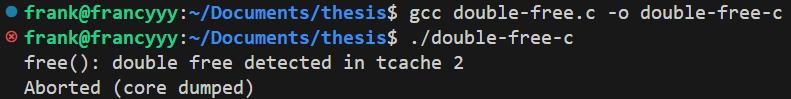
\includegraphics[width=1.0\textwidth]{double-free-c-exec}
    \caption{\textit{Double free} in C}\label{c:double-free-exec}
    \end{center}
\end{figure}
\begin{figure}[htbp]
\begin{center}
    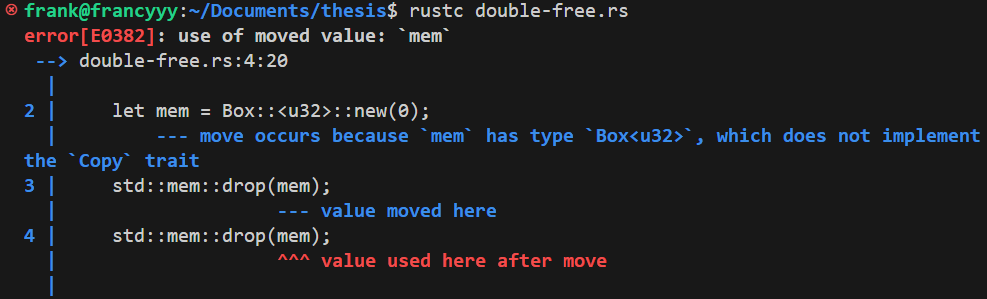
\includegraphics[width=1.0\textwidth]{double-free-rust-compile}
    \caption{Tentativo di \textit{double free} in Rust}\label{rust:double-free-compile}
    \end{center}
\end{figure}

% Dangling pointer
\subsubsection{Dangling pointers}
Un \textit{dangling pointer} (puntatore pendente) è un puntatore che riferisce a una locazione di memoria non più valida o che è stata liberata. 
Generalmente si presenta quando un'area di memoria viene deallocata, ma gli eventuali puntatori che la referenziavano non vengono aggiornati.

Si consideri l'esempio C riportato nel Listato~\ref{c:dangling-pointer} che genera un \textit{dangling pointer}\footnote{La presenza di uno scope interno non è funzionale all'esempio, ma non ne modifica nemmeno il risultato. È presente per garantire somiglianza strutturale con l'esempio Rust successivo.}:
\begin{lstlisting}[language=C, caption={Dangling pointer in C}, label={c:dangling-pointer}]
int main(void) {
    int* ptr;
    {
        int* val = malloc(sizeof(int));
        *val = 30;
        ptr = val;
        free(val);
    }
}
\end{lstlisting}
Nel listato~\ref{c:dangling-pointer}, viene allocata memoria sufficiente per un intero e il suo indirizzo è memorizzato 
sia in \texttt{val} che in \texttt{ptr}. La memoria viene successivamente deallocata invocando la funzione \texttt{free} sul puntatore \texttt{val}.
Tuttavia, il puntatore \texttt{ptr} non viene aggiornato, continuando a riferire alla stessa area di memoria, ormai non più valida.

È importante osservare che la sola esistenza un un \textit{dangling pointer} non causa un errore immediato.
Il comportamento indefinito si manifesta solo quando si tenta di derefenziare tale puntatore, cercando di leggere o scrivere nella memoria a cui fa riferimento. \hfill
\vspace{12pt}\\
\noindent A dimostrazione di ciò, si consideri che Rust permette la creazione di una \textit{dangling reference}, a patto che non venga utilizzata.
Il Listato~\ref{rust:dangling-pointer} mostra questa possibilità.
\begin{lstlisting}[language=Rust, caption={Dangling reference in Rust}, label={rust:dangling-pointer}]
fn main() {
    let _ref: &u32;
    {
        let val = Box::<u32>::new(30);
        _ref = &*val;
    }
}
\end{lstlisting}
Il listato~\ref{rust:dangling-pointer} tenta di replicare, per quanto possibile, il comportamento descritto nel listato~\ref{c:dangling-pointer}:
alla variabile \texttt{\_ref} viene assegnato un riferimento a \texttt{val}, allocata dinamicamente in uno scope interno. All'uscita 
da tale scope, \texttt{val} viene deallocato, lasciando \texttt{\_ref} con un riferimento non valido. 

Nonostante ciò, il compilatore non genera alcun errore.
Questo comportamento è giustificato dal fatto che la reference non è mai utilizzata\footnote{Il \textit{Borrow Checker} lavora in maniera \textit{lazy}: non verifica 
le condizioni di \textit{borrowing} e \textit{lifetime} di una reference fino a che non viene utilizzata.} e, di conseguenza, il \textit{Borrow Checker} non rileva alcuna
 violazione delle regole di \textit{borrowing}.

% Access after free
\subsubsection{Access after free}
Sebbene la sola presenza di un \textit{dangling pointer} non causi immediatamente problemi, essa rappresenta una condizione necessaria 
per un errore più grave: la \textit{access after free} (accesso post-liberazione).
Questo errore si verifica quando si tenta di accedere a memoria precedentemente deallocata, dereferenziando un \textit{dangling pointer}. 

A seconda del tipo
di accesso, si possono avere conseguenze differenti:
\begin{itemize}
    \item \textbf{Lettura}: può causare il recupero di dati non validi o incoerenti, eventualmente sovrascritti da allocazioni successive;
    \item \textbf{Scrittura}: può compromettere l'integrità della memoria, causando comportamenti indefiniti o crash del programma.
\end{itemize}
Nel Listato~\ref{c:access-after-free} è riportato un esempio C che, estendendo il listato~\ref{c:dangling-pointer}, genera un errore di \textit{access after free}:
\begin{lstlisting}[language=C, caption={Access after free in C}, label={c:access-after-free}]
#include <stdlib.h>
#include <stdio.h>
int main(void) {
    int* ptr;
    {
        int* val = malloc(sizeof(int));
        *val = 30;
        ptr = val;
        free(val);
    }
    printf("%d\n", *ptr);
}
\end{lstlisting}
Nel listato~\ref{c:access-after-free} si tenta di dereferenziare il puntatore \texttt{ptr} dopo che la memoria a cui faceva riferimento è stata deallocata.
In questo caso, l'accesso avviene per effettuare un'operazione di lettura, che rappresenta una forma
 meno distruttiva rispetto a una scrittura, ma che resta comunque pericolosa:
i dati letti potrebbero essere non validi o casuali, in quanto la memoria potrebbe essere stata sovrascritta da allocazioni successive.
 
Questo comportamento rappresenta un esempio di \textit{undefined behaviour}, come illustrato
dall'immagine~\ref{c:access-after-free-exec}. \hfill
\vspace{12pt}\\
\noindent Nel Listato~\ref{rust:rust-access-after-free} è riportato un programma che mostra come Rust gestisce questa problematica.
Per mantenere una somiglianza strutturale con la controparte C, il listato estende il precedente esempio riportato nel Listato~\ref{rust:dangling-pointer}.
\begin{lstlisting}[language=Rust, caption={Tentativo di \textit{access after free} in Rust}, label={rust:access-after-free}]
fn main() {
    let _ref: &u32;
    {
        let val = Box::<u32>::new(30);
        _ref = &*val;
    }
    println!("{}", _ref);
}
\end{lstlisting}
Il listato~\ref{rust:dangling-pointer} tenta di replicare il comportamento del listato~\ref{c:access-after-free}, cercando 
di accedere a una reference pendente per un'operazione di lettura.

Tuttavia, in questo caso viene generato un errore di compilazione, come mostrato in Figura~\ref{rust:access-after-free-compile}.
Il \textit{Borrow Checker} rileva che \texttt{\_ref} viene utilizzata successivamente alla deallocazione di \texttt{val}, rappresentando una violazione 
delle regole di \textit{borrowing} e, di conseguenza, impedisce la compilazione.
\begin{figure}[htbp]
\begin{center}
    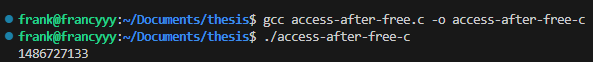
\includegraphics[width=.8\textwidth]{access-after-free-c-exec}
    \caption{\textit{Access after free} in C}\label{c:access-after-free-exec}
    \end{center}
\end{figure}
\begin{figure}[htbp]
\begin{center}
    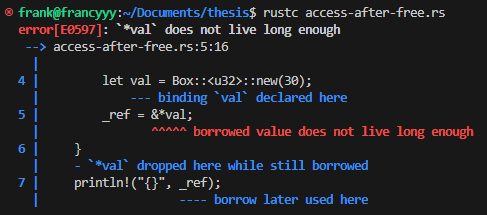
\includegraphics[width=.8\textwidth]{access-after-free-rust-compile}
    \caption{Tentativo di \textit{access after free} in Rust}\label{rust:access-after-free-compile}
    \end{center}
\end{figure}

% Buffer Overflow e Overread
\subsubsection{Access out of bounds: buffer overflow e overread}
L' \textit{access out of bounds} è un errore comune associato alla gestione manuale della memoria dinamica.
Si verifica quando si tenta di accedere a una porzione di memoria al di fuori dei limiti dell'area effettivamente allocata.

In base al tipo di accesso si distingue in due varianti: nel caso di una lettura si parla di \textit{buffer overread} 
(lettura oltre i limiti) mentre, nel caso di una scrittura, di \textit{buffer overflow} (sovraccarico o sovrascrittura del buffer).

\paragraph{Buffer overflow}
L'esempio riportato nel Listato~\ref{c:buffer-overflow} mostra un programma in C che genera un errore di \textit{buffer overflow}.
\begin{lstlisting}[language=C, caption={Buffer overflow in C}, label={c:buffer-overflow}]
#include <stdlib.h>
#include <stdio.h>
int main(void) {
    int* vec = malloc(sizeof(int) * 3);
    printf("Allocato un vettore di 3 interi, indici validi: 0, 1, 2\n");
    for(int i = 0; i <= 3; i++) {
        printf("Memorizzando %d all'indice %d\n", i * 10, i);
        vec[i] = i * 10;
    }
    free(vec);
    printf("Terminata la memorizzazione!\n");
    return 0;
}
\end{lstlisting}
Nel listato~\ref{c:buffer-overflow} viene allocata memoria suffiente per un vettore di tre interi, ma successivamente vengono
inizializzati quattro elementi, dall'indice \texttt{0} fino a \texttt{3}.
In questo caso il programma termina senza errori, viene anche eseguita la stampa finale, come mostrato dall'immagine~\ref{c:buffer-overflow-exec}. 

Nonostante ciò, questo comportamento non può essere considerato una garanzia in quanto, generalmente, la conseguenza di un \textit{buffer overflow} è un \textit{undefined behaviour}: 
non è possibile determinare a priori cosa contenga la memoria oltre
il limite dell'allocazione o per cosa venga utilizzata\footnote{In generale un \textit{buffer overflow} avviene all'interno dello spazio
di indirizzamento virtuale di un processo. In questo caso, la memoria potenzialmente corrotta sarebbe
 del processo stesso. Tuttavia, nel caso in cui l'indirizzo di riferimento
 fosse al di fuori dello spazio di indirizzamento virtuale del processo verrebbe generato un'errore runtime di tipo \textit{segmentation fault}, 
 causando l'immediato crash del programma.}. \hfill
\vspace{10pt}\\
\noindent Nel Listato~\ref{rust:buffer-overflow} è riportato un programma in Rust che mostra come viene gestito questo errore.
\begin{lstlisting}[language=Rust, caption={Buffer overflow in Rust}, label={rust:buffer-overflow}]
fn main() {
    let mut vec: Vec<u32> = vec![0; 3];
    println!("Allocato un vettore di 3 interi, indici validi: 0, 1, 2");
    for i in 0u32..=3u32 {    
        println!("Memorizzando {} all'indice {}", i * 10, i);
        vec[i as usize] = i * 10;
    }
    println!("Terminata la memorizzazione!");
}
\end{lstlisting}
Il listato~\ref{rust:buffer-overflow} tenta di replicare il comportamento del listato~\ref{c:buffer-overflow}, 
allocando un vettore di tre interi e successivamente cercando di inizializzarne quattro. 
In questo caso la compilazione va a buon fine, ma la stampa finale non avviene: il programma genera un \textit{panic} durante l'esecuzione. Questo avviene
durante l'accesso all'indice \texttt{3}, come mostrato in Figura~\ref{rust:buffer-overflow-exec}.

Questo comportamento è dovuto al fatto che il compilatore inserisce controlli di validità sugli indici, i quali vengono eseguiti a runtime.\footnote{Infatti, il compilatore non può sapere a tempo di compilazione quali saranno gli indici che verranno utilizzati per accedere a un vettore, quindi si limita a inserire controlli sulla loro validità prima degli accessi effettivi.}
\begin{figure}[htbp]
\begin{center}
    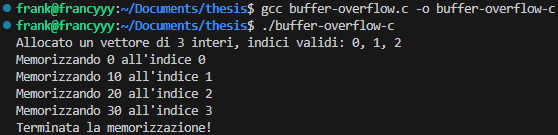
\includegraphics[width=.8\textwidth]{c-buffer-overflow-exec}
    \caption{\textit{Buffer overflow} in C}\label{c:buffer-overflow-exec}
    \end{center}
\end{figure}
\begin{figure}[htbp]
\begin{center}
    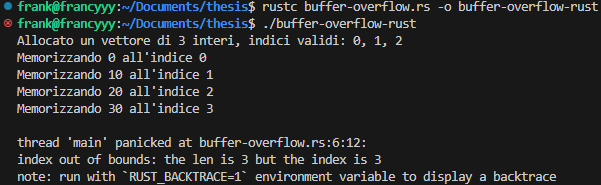
\includegraphics[width=.8\textwidth]{rust-buffer-overflow-exec}
    \caption{\textit{Buffer overflow} in Rust}\label{rust:buffer-overflow-exec}
    \end{center}
\end{figure}


\paragraph{Buffer overread}
L'esempio riportato nel Listato~\ref{c:buffer-overread} mostra un programma in C che genera un errore di \textit{buffer overread}.
\begin{lstlisting}[language=C, caption={Buffer overread in C}, label={c:buffer-overread}]
#include <stdlib.h>
#include <stdio.h>
int main(void) {
    int* vec = malloc(sizeof(int) * 3);
    for(int i = 0; i < 3; i++) vec[i] = i * 10;
    printf("Contenuto del vettore:\n");
    for(int i = 0; i < 10; i++)
        printf("Indice: %d -> Valore: %d\n", i, vec[i]);
    free(vec);
    return 0;
}
\end{lstlisting}
Nel listato~\ref{c:buffer-overread} viene allocata memoria per un vettore di tre interi, i quali vengono correttamente inizializzati e, successivamente,
si tenta di leggere dieci elementi dal vettore.
In questo caso il programma termina senza errori, stampando effettivamente dieci elementi, come mostrato dall'immagine~\ref{c:buffer-overread-exec}. 

Come quanto detto per l'errore di \textit{buffer overflow}, generalmente la conseguenza è un \textit{undefined behaviour}: 
non è possibile determinare a priori cosa contenga la memoria (oltre
il limite dell'allocazione) che viene letta\footnote{Vangono le stesse considerazioni fatte per il \textit{buffer overflow}: un'accesso a un indirizzo
che eccede lo spazio di indirizzi virtuali del processo genera un errore runtime di tipo \textit{segmentation fault}, causando l'immediato crash del programma}.\hfill
\vspace{10pt}\\
\noindent Rust gestisce questo errore in maniera analoga al \textit{buffer overflow}. Nel Listato~\ref{rust:buffer-overflow} è riportato un programma in Rust che mostra tale somiglianza.
\begin{lstlisting}[language=Rust, caption={Buffer overread in Rust}, label={rust:buffer-overread}]
fn main() {
    fn main() {
    let vec: Vec<u32> = vec![0, 10, 20];
    println!("Contenuto del vettore:");
    for i in 0..10 {
        println!("Indice: {} -> Valore: {}", i, vec[i]);
    }
}
}
\end{lstlisting}
Il listato~\ref{rust:buffer-overread} tenta di replicare il comportamento del listato~\ref{c:buffer-overread}, 
allocando un vettore di tre interi e successivamente cercando di leggerne dieci. 

Anche in questo caso la compilazione termina correttamente ma, durante l'esecuzione, in particolare durante l'accesso al quarto elemento, viene generato
un \textit{panic}. Questo comportamento può essere osservato in Figura~\ref{rust:buffer-overread-exec}.
\begin{figure}[htbp]
\begin{center}
    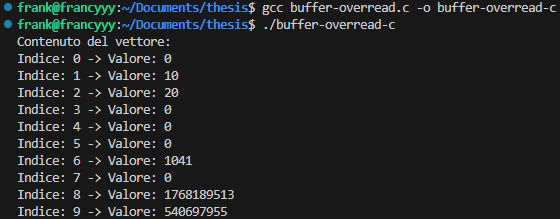
\includegraphics[width=.8\textwidth]{c-buffer-overread-exec}
    \caption{\textit{Buffer overread} in C}\label{c:buffer-overread-exec}
    \end{center}
\end{figure}
\begin{figure}[htbp]
\begin{center}
    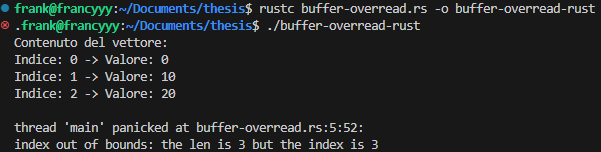
\includegraphics[width=.8\textwidth]{rust-buffer-overread-exec}
    \caption{\textit{Buffer overread} in Rust}\label{rust:buffer-overread-exec}
    \end{center}
\end{figure}

% Unitialized memory access
\subsubsection{Unitialized memory access} 
La \textit{unitialized memory access} (accesso a memoria non inizializzata) è un errore che si presenta
 quando si tenta di leggere da un'area di memoria che non è stata 
 inizializzata. Questo può portare a comportamenti imprevedibili, in quanto 
 i dati letti potrebbero essere casuali e potenzialmente 
 residui da allocazioni precedenti.

Nel linguaggio C, questo errore si presenta tipicamente quando viene 
allocata memoria tramite la funzione \texttt{malloc} e successivamente si tenta di 
accedervi senza previa inizializzazione.

Nel Listato~\ref{c:uninitialized-memory-access} viene riportato un esempio minimale C che genera un errore di questo tipo.
\begin{lstlisting}[language=C, caption={Uninitialized memory access in C}, label={c:uninitialized-memory-access}]
#include <stdlib.h>
#include <stdio.h>
int main(void) {
    int* ptr = malloc(sizeof(int));
    printf("%d\n", *ptr);
    free(ptr);
    return 0;
}
\end{lstlisting}
Nel listato~\ref{c:uninitialized-memory-access} viene allocata memoria sufficiente a contenere un intero e, senza inizializzarne il contenuto,
viene tentato un accesso in lettura. 
Il risultato è un comportamento indefinito: il valore letto potrebbe variare in base all'ambiente di esecuzione e tra esecuzioni, senza garanzia di coerenza.

È possibile osservare un caso particolare, in cui l'accesso può sembrare produrre un risultato coerente, come mostrato in Figura~\ref{c:uninitialized-memory-access-exec}\footnote{L'esecuzione è avvenuta su Ubuntu LTS 24.04 con \texttt{glibc}. In questo contesto è possibile che \texttt{malloc} azzeri la memoria allocata, prima di restituirne l'indirizzo, ma non è un comportamento garantito dallo standard C.}.
Tuttavia, questa apparente stabilità non può essere considerata una garanzia, in quanto vi sono più fattori che possono influenzare il valore letto:
\begin{itemize}
    \item Implementazioni specifiche dell'allocatore di memoria, che possono inizializzare la memoria allocata a zero o a un valore casuale;
    \item La posizione in memoria scelta dall'allocatore per il puntatore;
    \item Eventuali valori residui da allocazioni precedenti;
    \item La mappatura tra pagine virtuali e fisiche da parte del sistema operativo.
\end{itemize}
A conferma dell'inaffidabilità, si consideri l'esempio nel Listato~\ref{c:uninitialized-memory-access-2}, che estende il listato~\ref{c:uninitialized-memory-access}.
\begin{lstlisting}[language=C, caption={Uninitialized memory access in C}, label={c:uninitialized-memory-access-2}]
#include <stdlib.h>
#include <stdio.h>
int main(void) {
    int* ptr = malloc(sizeof(int));
    free(ptr);
    ptr = malloc(sizeof(int));
    printf("%d\n", *ptr);
    free(ptr);
    return 0;
}
\end{lstlisting}
Il listato~\ref{c:uninitialized-memory-access-2} mostra come eseguire una \texttt{free} prima della \texttt{malloc} successiva può lasciare residui nella memoria. 
Di conseguenza il valore letto, questa volta, è diverso da zero, come si può osservare dall'immagine~\ref{c:uninitialized-memory-access-exec-2}\footnote{Anche in questo caso, si tratta di un comportamento specifico del sistema e non garantito dallo standard.}.
\begin{figure}[htbp]
\begin{center}
    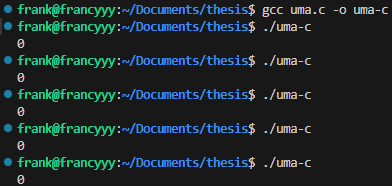
\includegraphics[width=.6\textwidth]{c-uninitialized-memory-access-exec}
    \caption{\textit{Uninitialized memory access} in C}\label{c:uninitialized-memory-access-exec}
    \end{center}
\end{figure}

\noindent Rust previene questa problematica in maniera strutturale, non permettendo allocazioni dinamiche senza inizializzazione grazie all'utilizzo di \texttt{smart pointers}, i quali prevedono un'inizializzazione obbligatoria.

In Rust infatti, le principali primitive per l'allocazione dinamica richiedono sempre l'inizializzazione dei valori:
\begin{itemize}
    \item \texttt{Box}: \textit{smart pointer} impiegato per allocare un singolo valore nella heap. L'unico modo per crearne uno è tramite \texttt{Box::new}, che richiede un valore per l'inizializzazione. In \textit{safe} Rust, non esiste un costrutto equivalente alla \texttt{malloc} in C;\ 
    \item \texttt{Vec}: \textit{smart pointer} utilizzato per una collezione dinamica di valori in heap. Anche se può essere creato vuoto (\texttt{Vec::new}), ogni accesso è verificato a runtime per evitare accessi oltre i limiti. In caso di violazioni viene generato un \textit{panic}, terminando l'esecuzione, come è osservabile in Figura~\ref{rust:buffer-overread-exec};
\end{itemize}
Di conseguenza, non è possibile sviluppare codice Rust che acceda a memoria non inizializzata senza ricorrere alla parola chiave \texttt{unsafe}\footnote{Rust consente l'accesso a memoria potenzialmente non inizializzata, ma soltanto all'interno di blocchi \textit{unsafe}. Un esempio è la funzione \texttt{std::mem::MaybeUninit}, ma meccanismi come questo sono riservati a casi particolari, in cui le garanzie di sicurezza devono essere gestite manualmente dal programmatore.}.
\begin{figure}[htbp]
\begin{center}
    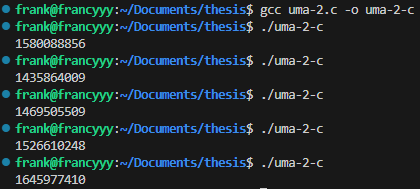
\includegraphics[width=.6\textwidth]{c-uninitialized-memory-access-exec-2}
    \caption{\textit{Uninitialized memory access} in C con previa \texttt{free}}\label{c:uninitialized-memory-access-exec-2}
    \end{center}
\end{figure}

\subsubsection{Conclusioni}
In conclusione, sotto l'aspetto della sicurezza della memoria, Rust si distingue da C garantendo un comportamento sicuro e deterministico, prevenendo
alcuni errori durante la compilazione e rilevandone altri a runtime. In C, d'altra parte, tali errori possono passare inosservati, causando
\textit{undefined behaviour} o crash del programma.

\subsection{Prestazioni}
In questa sottosezione verranno confrontate le prestazioni tipiche dei programmi scritti in C e Rust, basandosi
su benchmark esistenti e pubblicamente disponibili.

Non verrano presentati né codice dettagliato né un'analisi sperimentale diretta, per i seguenti motivi: una valutazione accurata
richiederebbe sviluppo di codice ottimizzato per entrambi i linguaggi, un set ampio di programmi da testare, differenti ambienti di esecuzione (diversi sistemi operativi, compilatori, architetture hardware) e una metodologia
di confronto rigorosa, che andrebbero oltre gli obiettivi di questa trattazione. \hfill
\vspace{10pt}\\
\noindent Come accennato a inizio del capitolo, il linguaggio C è storicamente noto per le prestazioni, principalmente in termini di velocità d'esecuzione, dovute all'assenza di astrazioni
complesse e al runtime minimo richiesto. 

Rust, d'altra parte, mira a garantire la sicurezza della memoria senza compromettere le prestazioni, puntando a fornire velocità d'esecuzione paragonabili a C e C++. \hfill
\vspace{10pt}\\
\noindent Per offrire un confronto concreto, vengono riportati i risultati tratti da \textit{The Computer Language Benchmarks Game}
\footnote{Nel sito vengono raccolti i risultati dell'esecuzione di vari algoritmi sviluppati in diversi linguaggi di programmazione. Il sito potrebbe variare nel tempo e
i risultati riportati nella trattazione potrebbero non essere più i migliori e peggiori (data di riferimento 2025-07-18)}~\cite{benchmarksgame}, un progetto che
confronta le prestazioni di diversi linguaggi di programmazione nell'esecuzione di algoritmi comuni. Il confronto si basa su quattro parametri:
\begin{itemize}
    \item \textbf{secs}: tempo di esecuzione totale (\textit{wall-clock time});
    \item \textbf{cpu secs}: tempo effettivo utilizzato dalla CPU, trascurando attese dovute a I/O e context switch;
    \item \textbf{mem}: picco di memoria RAM utilizzata dal processo;
    \item \textbf{gz}: dimensione del file sorgente compresso con \texttt{gzip}, interpretato come indice di verbosità e complessità dell'implementazione.
\end{itemize}
Verranno analizzati due benchmark distinti: uno principalmente \textit{CPU-bound} e uno principalmente \textit{I/O-bound}. 
Non viene incluso un esempio della categoria `\textit{contentious}', in quanto tali benchmark tendono a essere influenzati 
da librerie esterne e dalla specifica implementazione degli algoritmi, non tanto dalle caratteristiche intrinseche del linguaggio e, per questo, 
non rientrano negli obiettivi della trattazione.

\subsubsection{Confronto CPU-bound}\label{par:cpu-bound} Il benchmark \textit{CPU-bound} considerato è \texttt{n-body}. Il problema consiste
nel simulare il moto di \texttt{n} corpi che interagiscono attraverso la forza gravitazionale:
a ogni passo viene calcolata la forza tra tutte le coppie di corpi,
si aggiornano le velocità in base alle accelerazioni risultanti e si aggiornano le posizioni.
L'algoritmo ha complessità quadratica (\texttt{O($n^2$)}) ed è privo di I/O significativo: è un carico interamente \textit{CPU-bound}. \hfill
\vspace{10pt}\\
\noindent Nella Tabella~\ref{tab:n-body} sono riportati i risultati del benchmark \texttt{n-body} relativi a Rust e C. 
Per ciascun linguaggio è stata selezionata l'esecuzione migliore e quella peggiore in termini di \textbf{cpu secs}. Sono state considerate solo 
le implementazioni ideomatiche, escludendo quelle che ricorrono a \textit{SIMD scritti a mano}\footnote{Si tratta di un'ottimizzazione manuale del codice per sfruttare le istruzioni vettoriali della CPU:\  invece di scrivere codice `standard', il programmatore scrive esplicitamente codice che utilizza i registri \textit{Single Instruction, Multiple Data}.} o a codice \textit{unsafe} in Rust. \hfill
\begin{table}[h]
    \centering
    \begin{tabular}{lcccc}
        \toprule
        \textbf{Linguaggio} & \textbf{secs} & \textbf{cpu secs} & \textbf{mem} (KB) & \textbf{gz} (B) \\
        \midrule
        Esecuzione migliore & & & & \\
        C  & 4.98 & 4.98 & 2482 & 1186 \\
        Rust & 3.46 & 3.46 & 2937 & 1774 \\
        \midrule
        Esecuzione peggiore & & & & \\
        C & 6.89 & 6.89 & 2490 & 1250 \\
        Rust & 5.52 & 5.51 & 3027 & 1483 \\
        \bottomrule
    \end{tabular}
    \caption{Risultati \texttt{n-body} per Rust e C (implementazioni ideomatiche)}
    \label{tab:n-body}
\end{table}
\vspace{1pt}\\
\noindent Dagli estratti riportati nella Tabella~\ref{tab:n-body} è possibile osservare che, da un punto di vista temporale, anche in un benchmark puramente \textit{CPU-bound},
Rust riesca a raggiungere C in termini di velocità d'esecuzione, senza ricorrere a codice \textit{unsafe}. 
Nei benchmark, Rust ha addirittura superato C in velocità d'esecuzione:
nel caso migliore, Rust ha impiegato
circa il \texttt{30\%} di tempo in meno; nel caso peggiore circa il \texttt{20\%}. 

Questo risultato supporta l'idea che Rust possa rappresentare un'alternativa a C anche in contesti ad alta intensità computazionale, pur garantendo la sicurezza della memoria.

Dal punto di vista dell'occupazione di risorse, invece, C si presenta vantaggioso, richiedendo una quantità inferiore di memoria durante l'esecuzione e producendo sorgenti più compatti (successivamente alla compressione).

\subsubsection{Confronto I/O-bound} Il benchmark \textit{I/O-bound} selezionato è \texttt{fasta}. Il problema consiste nella generazione di DNA (utilizzando i caratteri \texttt{A}, \texttt{C}, \texttt{G} e \texttt{T}) secondo pattern sia deterministici che pseudocasuali, seguita dalla 
loro scrittura sullo standard output. 
L'algoritmo presenta un carico di elaborazione minimo: rappresenta un esempio di algoritmo principalmente \textit{I/O-bound}, in quanto la maggior parte del tempo di esecuzione è trascorso in scrittura sullo standard output.
Inoltre, la presenza di generazione pseudocasuale e ripetitiva comporta un utilizzo intensivo di stringhe e buffer, rendendo il benchmark utile per verificare l'efficienza di gestione della memoria dinamica. \hfill
\vspace{7pt}\\
\noindent Nella Tabella~\ref{tab:fasta} sono riportati i risultati del benchmark \texttt{fasta} relativi a Rust e C.
Come specificato nell'analisi CPU-bound~\ref{par:cpu-bound}, per ciascun linguaggio viene riportata l'esecuzione migliore e quella peggiore in termini di \textbf{cpu secs}. Sono state considerate solamente
le implementazioni ideomatiche, escludendo quelle che ricorrono a \textit{SIMD scritti a mano} o codice \textit{unsafe} in Rust.
\begin{table}[h]
    \centering
    \begin{tabular}{lcccc}
        \toprule
        \textbf{Linguaggio} & \textbf{secs} & \textbf{cpu secs} & \textbf{mem} (KB) & \textbf{gz} (B) \\
        \midrule
        Esecuzione migliore & & & & \\
        C & 0.79 & 0.78  & 2236 & 1469\\
        Rust & 2.03 & 2.03 & 3199 & 1235 \\
        \midrule
        Esecuzione peggiore & & & & \\
        C & 8.27 & 8.27 & 2195 & 839 \\
        Rust & 4.45 & 4.45 & 3113 & 1240 \\
        \bottomrule
    \end{tabular}
    \caption{Risultati del benchmark fasta per Rust e C (implementazioni ideomatiche)}
    \label{tab:fasta}
\end{table}
\vspace{6pt}\\
\noindent Dai risultati mostrati nella Tabella~\ref{tab:fasta} si osserva che non emerge un chiaro vantaggio costante tra i due linguaggi:
nel caso migliore, C è circa \texttt{2.6} volte più veloce di Rust, mentre nel caso peggiore è Rust a richiedere circa la metà del tempo rispetto a C.

\noindent Dal punto di vista dell'occupazione di risorse, valgono ancora le considerazioni fatte durante l'analisi \textit{CPU-bound}: C, generalmente, richiede una quantità minore di memoria RAM durante l'esecuzione e
produce sorgenti più contenuti (una volta compressi), indicando una complessità minore dell'implementazione.

\subsubsection{Conclusione} 
Dai risultati analizzati emerge che entrambi i linguaggi offrono prestazioni paragonabili, con differenze che variano in base al tipo di carico e all'implementazione specifica.

Con le opporture ottimizzazioni, sia 
a livello di scrittura del codice che di compilazione, Rust è in grado di raggiungere, e in alcuni casi superare, le prestazioni di C in termini di velocità d'esecuzione, pur garantendo sicurezza della memoria. \hfill
\vspace{5pt}\\
\noindent Tuttavia, un evidente svantaggio di Rust è rappresentato dagli elevati tempi di compilazione, specialmente rispetto a C, dovuti principalmente ai controlli effettuati dal \textit{Borrow Checker} per determinare, e verificare, le relazioni di \textit{ownership} e \textit{borrowing}.
Questo overhead in fase di compilazione è però compensato dalla sicurezza della memoria, garantita a tempo di compilazione, non richiedendo overhead aggiuntivi durante l'esecuzione. \hfill
\vspace{5pt}\\
\noindent Dal punto di vista della dimensione dei file eseguibili, Rust tende a generare file di dimensioni maggiori, principalmente per l'inclusione della libreria standard e dei simboli di debug\footnote{Tramite le opzioni del compilatore è possibile indicare l'ottimizzazione per lo spazio, che cerca di ridurre le dimensioni dell'eseguibile. Inoltre, in contesti di programmazione \textit{bare-metal}, è possibile escludere la libreria standard (\#![no\_std]), in quanto non è presente un sistema operativo sottostante.}. \hfill
\vspace{5pt}\\
\noindent Infine, per quanto riguarda l'utilizzo della memoria durante l'esecuzione, entrambi i linguaggi mostrano requisiti simili, con Rust che, tendenzialmente, può richiedere una quantità leggermente superiore di RAM, dovuta principalmente all'utilizzo di astrazioni.
Infatti, nonostante quest'ultime siano definite \textit{zero-cost} in teoria, nella pratica, spesso, il compilatore non riesce a ottimizzarle pienamente e possono introdurre un minimo overhead.

\subsection{Complessità del codice}
Una critica comune nei confronti di Rust, specialmente da coloro che provengono da C, è la maggiore complessità e verbosità del linguaggio.
Generalmente, la sintassi di C è considerata più semplice e minimale, principalmente per la sua natura a basso livello, la mancanza di astrazioni
complesse e la presenza di un numero limitato di costrutti.

Al contrario in Rust, dovendo gestire attentamente le relazioni di \textit{ownership}, \textit{borrowing} e \textit{lifetime}, il codice può risultare più complesso; 
questi non sono gli unici aspetti che contribuiscono a questa percezione: gestione degli errori, controllo del flusso, supporto a \textit{generics} e \textit{macro} sono
tutti elementi che possono rendere il linguaggio più verboso e complesso rispetto a C.

\subsubsection{Annotazioni di lifetime}
Una delle principali differenze tra Rust e C è dovuta alla presenza del \textit{modello di ownership}, che impone annotazioni di \textit{lifetime} nei casi in cui non siano deducibili implicitamente.
Come già accennato nel capitolo tre: `\textit{Sistemi Operativi}'~\ref{cap:03}, queste permettono al \textit{Borrow Checker} di determinare la validità di un prestito nel tempo, rifiutando 
codice che viola le annotazioni.

Queste annotazioni introducono un livello ulteriore di complessità, sia sintattica che contettuale: il programmatore deve specificare quanto a lungo
un riferimento sarà valido, dovendo ragionare in termini di durata dei dati nel tempo.

Tuttavia, la complessità viene compensata da una maggiore sicurezza del codice: come verrà mostrato successivamente, permette di prevenire
problemi quali \textit{access after free}. \hfill
\vspace{10pt} \\
\noindent In C questo meccanismo non è presente, non esiste proprio il concetto di \textit{lifetime} come elemento del linguaggio. In questi
casi è il programmatore che deve garantire che i puntatori siano validi, senza supporto da parte del linguaggio.

Nei Listati~\ref{rust-lifetime-prevention} e~\ref{c:lifetime-prevention} verranno riportati due esempi che mostrano come le annotazioni di \textit{lifetime} possano prevenire \textit{access after free}.
\begin{lstlisting}[language=Rust, caption={Prevenzione di \textit{access after free} tramite \textit{lifetime annotations}}, label={rust:lifetime-prevention}]
fn biggest<'a>(a: &'a i32, b: &'a i32) -> &'a i32 {
    if *a > *b { a } else { b }
}
fn main (){
    let result;
    let smaller = Box::<i32>::new(1);
    {
        let bigger = Box::<i32>::new(2);
        result = biggest(&*smaller, &*bigger);
    }
    println!("Il piu grande e: {}", *result);
}
\end{lstlisting}
\begin{lstlisting}[language=C, caption={\textit{Access after free} dovuta alla mancanza di \textit{lifetime} in C}, label={c:lifetime-prevention}]
#include <stdlib.h>
#include <stdio.h>
int* biggest(int* a, int* b) {
    return (*a > *b) ? a : b;
}
int main(void) {
    int* result;
    int* smaller = malloc(sizeof(int));
    *smaller = 1;
    {
        int* bigger = malloc(sizeof(int));
        *bigger = 2;
        result = biggest(smaller, bigger);
        free(bigger);
    }
    printf("Il piu grande e: %d\n", *result);
    free(smaller);
}
\end{lstlisting}
Entrambi i listati,~\ref{rust:lifetime-prevention} e~\ref{c:lifetime-prevention}, implementano la stessa logica: definiscono una funzione \texttt{biggest} che
riceve in ingresso due riferimenti (o puntatori, nel caso di C) e restituisce quello che punta al valore maggiore.
La funzione \texttt{main} alloca due interi, \texttt{smaller} e \texttt{bigger}, nella heap e passa un riferimento a ciascuno a 
\texttt{biggest}.
Per come sono inizializzati, la funzione restituisce un rifermento a \texttt{bigger}. Tuttavia, \texttt{bigger} viene deallocato prima della stampa, lasciando un \textit{dangling pointer}.

Qua è possibile osservare la differenza tra i due linguaggi:
\begin{itemize}
    \item In C, il compilatore produce un eseguibile senza generare alcun avviso o errore. L'esecuzione sembra funzionare, ma in realtà viene generato un \textit{access after free}, leggendo un valore corrotto, come illustrato in Figura~\ref{c:aaf-lifetime};
    \item In Rust, invece, \texttt{biggest} specifica una sola \textit{lifetime}, \texttt{'a}, indicando che tutte le reference (le due in ingresso e quella in uscita) devono essere valide per la durata di tale \textit{lifetime}. Il \textit{Borrow Checker} rileva che \texttt{smaller} e \texttt{bigger}, essendo definiti in scope differenti, hanno \textit{lifetime} diverse e impedisce la compilazione. È possibile osservare questo comportamento in Figura~\ref{rust:aaf-lifetime}.
\end{itemize}
\begin{figure}[htbp]
    \begin{center}
        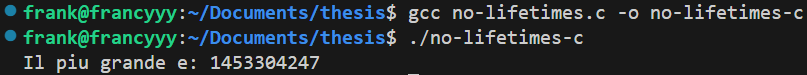
\includegraphics[width=.9\textwidth]{c-aaf-lifetime}
        \caption{\textit{Access after free} dovuto all'assenza di \textit{lifetime} in C}\label{c:aaf-lifetime}
    \end{center}
\end{figure}
\begin{figure}[htbp]
    \begin{center}
        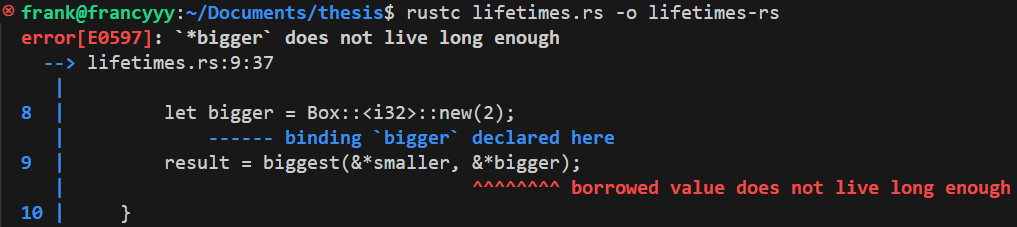
\includegraphics[width=.9\textwidth]{rust-aaf-lifetime}
        \caption{Tentativo di {access after free} in Rust}\label{rust:aaf-lifetime}
    \end{center}
\end{figure}
Questo è un esempio che mostra come Rust, tramite le annotazioni di \textit{lifetime}, presenti una sintassi più complessa rispetto a C, ma allo stesso tempo più sicura.

\subsubsection{Generics}
Le espressioni \textit{generics} o \textit{generic programming} indicano un meccanismo di astrazione che consente di sviluppare codice indipendente da un tipo di dato specifico.
Il tipo viene fornito come argomento, generalmente in fase di compilazione, consentendo il riuso del codice con diversi tipi di dato. \hfill
\vspace{8pt}\\
\noindent Il linguaggio C non supporta nativamente lo sviluppo di codice parametrico, in quanto comporterebbe un livello di astrazione superiore rispetto alla
semplicità a cui il linguaggio aspira. Nonostante ciò, è possibile emulare un comportamento simile, principalmente tramite l'uso di puntatori \texttt{void*}, i quali possono riferirsi a valori di qualunche tipo.
Questo meccanismo, per quanto flessibile, richiede controlli rigorosi da parte del programmatore: 
\begin{itemize}
    \item un puntatore \texttt{void*} non memorizza informazioni sulla dimensione del valore puntato, rendendo necessaria la conoscenza esplicita del tipo (solitamente memorizzandone la dimensione);
    \item le operazioni di accesso, sia in lettura che scrittura, devono essere effettuate tramite funzioni delicate come \texttt{memcpy}, in quanto non è possibile dereferenziare direttamente un puntatore \texttt{void*}.
\end{itemize}
Il listato~\ref{c:generics} riporta un'estratto da un'implementazione in C di un nodo di una lista generica. L'implementazione completa è disponibile sulla piattaforma Github\footnote{Disponibile nel repository, \href{https://github.com/whocaresleft/C-data-structures}{\texttt{C-data-structures}}, personale del candidato, seguendo il percorso: \texttt{src/linear/}. Alcuni commenti sono stati rimossi o spostati per ragioni di spazio.}~\cite{github-ds-repo}.
\begin{lstlisting}[language=C, float, caption={Programmazione generica in C}, label={c:generics}]
typedef struct clinkedlist {
	node* tail;
	size_t element_count; /* Number of elements present in the list */
	size_t element_size; /* Size of the elements stored in the list */
} clinkedlist;

typedef struct node {
	void* ptr; /* Pointer to the memory location that stores the node's value */
	node* next; /* Pointer to the next node */
} node;

node* node_create(void* value, size_t value_size) {

	node* n = NULL;
	if (value_size <= SIZE_MAX) {

		n = (node*)malloc(sizeof(node));
		if (n) {

			n->ptr = malloc(value_size);
			if (n->ptr) {

				memcpy(n->ptr, value, value_size);
				n->next = NULL;
			}
			else {
				free(n);
				n = NULL;
			}
		}
	}
	return n;
}
\end{lstlisting}
Nell'implementazione di riferimento sono state adottate alcune strategie per cercare di prevenire errori legati alla gestione manuale dei tipi e della memoria:
\begin{itemize}
    \item \textbf{Tipo opaco}: la struttura dati è definita solo nel file sorgente, mentre l'header contiene solo una dichiarazione incompleta (\textit{opaque type}). Questo impedisce l'accesso diretto ai campi, tra cui \texttt{element\_size} di \texttt{clinkedlist}, la cui integrità è fondamentale per il corretto funzionamento della struttura;
    \item \textbf{Incapsulamento parziale}: la manipolazione della struttura è possibile solo tramite le funzioni fornite, obbligando l'utente a seguire un percorso logico e controllato per l'inserimento, la rimozione e la lettura dei dati. Questo permette l'introduzione di controlli interni riguardanti la validità e la coerenza dei dati. 
\end{itemize}
Nonostante queste precauzioni, il modello rimane fragile, per via della natura del linguaggio: l'utilizzo di \texttt{void*} permette la memorizzazione di qualsiasi valore, tra cui anche, altri puntatori; tuttavia, una eccessiva stratificazione di indirezione (in altre parole,\  puntatori a puntatori) può compromettere
la corretta deallocazione della memoria. \hfill
\vspace{15pt} \\
\noindent Rust adotta un approccio diverso, supportando la programmazione generica tramite le cosiddette \textit{zero-cost abstractions}\footnote{Si tratta di meccanismi e implementazioni astratti che non introducono overhead in fase di esecuzione rispetto al codice esplicito (concreto) equivalente.}.
Durante la fase di compilazione, il compilatore applica un processo detto \textit{monomorfizzazione}, trasformando ogni utilizzo di una funzione o una struttura
generica in una versione specifica per il tipo utilizzato.\hfill 
%Rust consente inoltre di specificare vincoli sui tipi generici (\textit{trait bounds}), tramite \texttt{impl Trait} e \texttt{where}. Questi meccanismi sono equivalenti, rispettivamente, a \texttt{implements Interface} e \texttt{<T extends \ldots>} di Java. \hfill
\vspace{8pt}\\
\noindent Per ottenere un confronto sulla complessità del codice, viene riportato, nel listato~\ref{rust:generics}, l'implementazione in Rust del listato~\ref{c:generics}: 
il supporto alla programmazione generica di Rust permette di definire strutture dati e funzioni generiche con codice sicuro e conciso.
\begin{lstlisting}[language=C, float, caption={Programmazione generica in Rust}, label={rust:generics}]
struct Clinkedlist<T> {
	tail: Option<Box<Node<T>>>,
	element_count: usize
}

struct Node<T> {
    value: T,
    next: Option<Box<Node<T>>>
}

impl<T> Node<T> {
    fn new(value: T) -> Node<T> {
        Node {
            value,
            next: None
        }
    }
}
\end{lstlisting}

L'implementazione risulta più semplice rispetto alla controparte C:\ non è necessario gestire manualmente la dimensione dei valori o gli accessi diretti alla memoria.
A tal proposito, si consideri che \texttt{Node::<T>::new()} del listato~\ref{rust:generics} è l'equivalente di \texttt{node\_create} del listato~\ref{c:generics}.

\subsubsection{Gestione degli errori}
I due linguaggi si distinguono per i meccanismi impiegati per la gestione degli errori.
In C, tipicamente, tale gestione è opzionale: il linguaggio non impone alcun controllo esplicito, lasciando la responsabilità al programmatore.
Il meccanismo maggiormente diffuso per segnalare errori è basato sul valore di ritorno, tipicamente interi, da parte delle funzioni, secondo
convenzioni informali e non uniformi\footnote{Lo standard C non definisce una convenzione uniforme sugli interi da utilizzare come codice di errore. Alcune funzioni
utilizzano 0 per indicare successo e ogni altro valore viene interpretato come fallimento. Per questo motivo, è sempre opportuno controllare la documentazione di una funzione,
per determinare come interpretare l'esito: alcune funzioni potrebbero intepretare ogni valore non negativo con successo, come altre potrebbero utilizzare 0 per fallimento.}.

L'assenza di vincoli espliciti sul controllo dell'esito rende facile, e comune, la mancata verifica di errori. 
Questo tuttavia può portare a comportamenti indefiniti, principalmente dovuti all'elaborazione di dati non validi, derivanti da
chiamate a funzioni fallite, il cui risultato viene interpretato come se fosse corretto. \hfill
\vspace{9pt}\\
\noindent Come riportato dalla documentazione ufficiale~\cite{rust-book}, Rust distingue tra due classi di errori, 
\textit{recuperabili} e \textit{irrecuperabili}, fornendo meccanismi distinti per la loro gestione.

Gli errori \textit{irrecuperabili} rappresentano situazioni dalle quali non è sicuro proseguire con l'esecuzione del programma, come l'accesso oltre i limiti di un array o 
il tentativo di dereferenziare un valore \texttt{None}\footnote{Rust utilizza l'enumerazione \texttt{Option<T>} per rappresentare un valore opzionale: \texttt{Some(T)} rappresenta la presenza di un valore, di tipo \texttt{T}, mentre \texttt{None} rapprenta l'assenza di un valore valido.}. 
Rust gestisce questo tipo di errore tramite \textit{panic}, i quali causano l'immediata interruzione del programma e rilasciano correttamente
tutte le risorse allocate dal processo.

Al contrario, gli errori \textit{recuperabili} rappresentano situazioni meno gravi, per le quali è possibile definire una logica di gestione, senza necessità di interruzione: per esempio, il tentativo di apertura di un file inesistente potrebbe essere gestito creando il file, invece di terminare l'esecuzione.
Per la gestione di questo tipo di errore Rust adotta l'enumerazione \texttt{Result<T, E>}.

A differenza del C, la gestione esplicita degli errori è obbligatoria in Rust: gli errori irrecuperabili vengono gestiti tramite \texttt{panic}; per quelli recuperabili, il 
compilatore impone al programmatore di gestire esplicitamente entrambe le varianti (\texttt{Ok} ed \texttt{Err}) tramite costrutti come \texttt{match} e \texttt{if let} oppure operatori come \texttt{?}, il quale propaga l'errore. 
Questo obbligo riduce la probabilità di errori non gestiti, rendendo il codice più sicuro e robusto rispetto all'approccio tradizionale di C.

\subsubsection{Macro}
I due linguaggi gestiscono le \textit{macro} in maniera completamente differente.
Come riportato dalla documentazione GCC~\cite{GNU-online-docs}, le \textit{macro} in C sono frammenti di codice a cui viene associato un nome, dichiarate con la direttiva \texttt{\#define}. 

Durante la fase di pre-processamento (prima della compilazione),
quando viene incontrato il nome di una \textit{macro}, esso viene sostituito con il codice associato. Si tratta di una semplice sostituzione testuale, come
mostrato nel Listato~\ref{c:macro}.
\begin{lstlisting}[language=C, caption={Definizione di \textit{macro} in C}, label={c:macro}]
#define printline(x) printf("%s\n", x)
int main(void) {
    printline("Stampa di prova");
    return 0;
}
\end{lstlisting}
Nel listato~\ref{c:macro}, viene definita la \textit{macro} \texttt{printline}, che stampa la stringa \texttt{x}, andando a capo successivamente.
All'interno della funzione main viene invocata `\texttt{printline("Stampa di prova")}': questa sarà espansa in `\texttt{printf("\%s\textbackslash n", "Stampa di prova")}' dal pre-processore. 

In quanto la sostituzione avviene durante la fase di pre-processamento,
per osservare il codice generato è necessario utilizzare il flag \texttt{-E} durante la compilazione con
 \texttt{GCC}\footnote{Tramite la opzione \texttt{-E} viene indicato a \texttt{GCC} di fermarsi dopo la fase di pre-processamento, 
 senza effettuare la compilazione. L'output della fase di pre-processamento verrà poi indirizzato allo standard output.}, 
 come mostrato in Figura~\ref{c:macro-preprocess}. \hfill
\begin{figure}[htbp]
    \begin{center}
        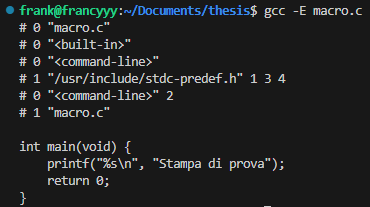
\includegraphics[width=.6\textwidth]{c-macro-preprocess}
        \caption{Traduzione di una \textit{macro} in C}\label{c:macro-preprocess}
    \end{center}
\end{figure}
La natura semplice delle macro C comporta delle limitazioni e falle di sicurezza, molte delle quali sono riportate sulla documentazione GCC~\cite{GNU-online-docs}. 
A dimostrazione di ciò, si consideri l'esempio riportato nel Listato~\ref{c:macro-2}, modifica del listato~\ref{c:macro}.
\begin{lstlisting}[language=C, caption={Utilizzo scorretto di \textit{macro} in C}, label={c:macro-2}]
#include <stdio.h>
#define printline(x) printf("%s\n", x)
int main(void) {
    int my_val = 150;
    printline(my_val);
    return 0;
}
\end{lstlisting}
Nel listato~\ref{c:macro-2} si tenta di sfruttare la stessa macro, \texttt{printline}, per stampare il contenuto di un intero. 
È interessante osservare che, nonostante il mismatch dei tipi (\texttt{\%s} indica di interpretare il parametro come stringa), il compilatore
 genera soltanto un warning, producendo lo stesso un file eseguibile. 
Tuttavia, tentando l'esecuzione si verifica un crash immediato dovuto a \textit{segmentation fault},
come è osservabile dall'immagine~\ref{c:macro-exec}. \hfill
\begin{figure}[htbp]
    \begin{center}
        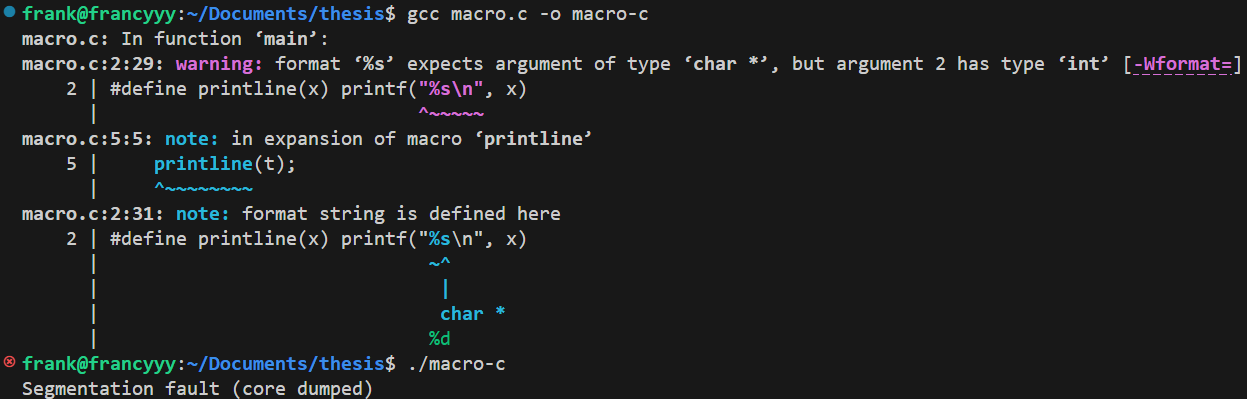
\includegraphics[width=1\textwidth]{c-macro-exec}
        \caption{Limitazioni delle \textit{macro} C}\label{c:macro-exec}
    \end{center}
\end{figure}
\vspace{10pt}\\
\noindent In Rust le \textit{macro} si distinguono in due classi: dichiarative e procedurali. Le \textit{macro} procedurali sono molto complesse e richiederebbero un capitolo
a parte, ma andrebbe oltre l'ambito di questa trattazione. 

Le \textit{macro} dichiarative, pur essendo meno complesse rispetto a quelle procedurali, sono caratterizzate comunque da una sintassi particolare,
basata su \textit{match di pattern}, permettendo
perfino l'\textit{overloading} in base al \textit{pattern} come riportato dalla documentazione ufficiale~\cite{rust-book}. 
Anche queste richiederebbero un capitolo 
dedicato per una spiegazione sufficientemente dettagliata. \hfill
\vspace{9pt}\\
\noindent Per mostrare la maggiore complessità, e differente gestione, delle \textit{macro} Rust rispetto alla controparte C, si consideri l'esempio rappresentativo\footnote{L'esempio fornito è basato su quello riportato nella documentazione ufficiale~\cite{rust-book}, nella sezione relativa all'overloading di macro.} nel Listato~\ref{rust:macro}.
\begin{lstlisting}[language=Rust, caption={Definizione di \textit{macro} dichiarativa in Rust}, label={rust:macro}]
macro_rules! comp_eval {
    ($sx:expr; and $dx:expr) => {
        println!(
            "{:?} and {:?} is {:?}",
            stringify!($sx), stringify!($dx), $sx && $dx
        )
    };
    ($sx:expr; or $dx:expr) => {
        println!(
            "{:?} or {:?} is {:?}",
            stringify!($sx), stringify!($dx), $sx || $dx
        )
    };
    ($not:expr) => {
        println!(
            "not {:?} is {:?}",
            stringify!($not), !($not)
        )
    };
}
fn main() {
    comp_eval!(1 + 2 == 3; and true);
    comp_eval!(true; or false);
    comp_eval!(true);
}
\end{lstlisting}
Nel listato~\ref{rust:macro} è definita la \textit{macro} dichiarativa \texttt{comp\_eval} che, in base al pattern, espande un codice diverso:
\begin{itemize}
    \item Se viene fornita una coppia di espressioni, \texttt{\$sx} e \texttt{\$dx}, separate dalla parola chiave \texttt{and}, la \textit{macro} espande una stampa della loro congiunzione logica;
    \item Se le espressioni sono separate dalla parola chiave \texttt{or}, espande una stampa della loro disgiunzione logica;
    \item Se invece viene fornita una singola espressione, \texttt{\$not}, la \textit{macro} espande una stampa della sua negazione logica.
\end{itemize}
Il risultato dell'esecuzione di questo codice è osservabile in Figura~\ref{rust:correct-macro}. \hfill
\vspace{0pt}\\
\noindent Le \textit{macro} Rust rappresentano uno strumento molto potente rispetto alle direttive pre-processore di C:\  permettono di definire comportamenti 
differenti in base alla struttura dell'invocazione, cosa non
possibile con la semplice sostituzione testuale.

Un'altra differenza rispetto alle \textit{macro} C riguarda la loro espansione: le \textit{macro} in Rust vengono espanse a livello di compilazione e in caso di mancata
corrispondenza con qualsiasi \textit{pattern} previsto viene generato un errore di compilazione.

Ad esempio, aggiungendo l'invocazione `\texttt{comp\_eval!("test")}' all'interno della funzione \texttt{main} nel listato~\ref{rust:macro}, si otterrà un errore
durante la compilazione in quanto il \texttt{pattern} fornito non corrisponde a nessuna delle regole definite nella macro\footnote{In questo esempio il pattern fornito è una singola stringa, quindi la regola adeguata sarebbe la terza, che accetta un'unica espressione. Tuttavia, l'operatore di negazione logica non può essere applicato a una stringa, di conseguenza il compilatore rifiuta il codice, generando un errore.}.
Il messaggio di errore è osservabile in Figura~\ref{rust:incorrect-macro}.
\begin{figure}[htbp]
    \begin{center}
        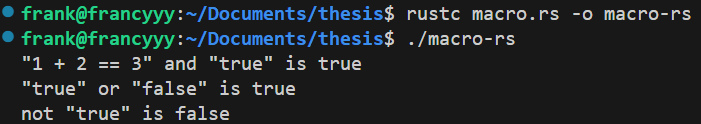
\includegraphics[width=.8\textwidth]{rust-correct-macro}
        \caption{Compilazione di una \textit{macro} in Rust}\label{rust:correct-macro}
    \end{center}
\end{figure}
\begin{figure}[htbp]
    \begin{center}
        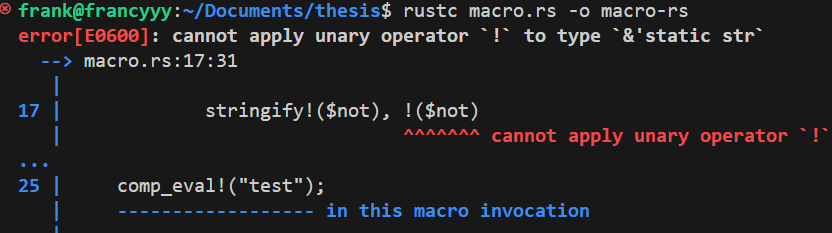
\includegraphics[width=.8\textwidth]{rust-incorrect-macro}
        \caption{Errore durante la compilazione di una \textit{macro} in Rust}\label{rust:incorrect-macro}
    \end{center}
\end{figure}

\subsubsection{Conclusioni}
Nonostante siano limitati, gli aspetti esaminati mettono in luce un tratto distintivo di Rust, specialmente rispetto a C:\ il linguaggio
richiede uno sforzo iniziale maggiore, dovuto alla maggiore complessità della sintassi, ma questo viene ripagato garantendo meccanismi 
di sicurezza della memoria affidabili e integrati nel linguaggio stesso.